\section{Implementación de Pruebas}

Para garantizar el correcto funcionamiento de la aplicación, durante el desarrollo se ha realizado una fase de pruebas. Principalmente se han implementado pruebas unitarias, pero también algunas pruebas de integración para verificar el comportamiento de ciertos componentes y su interaccion con los componentes vecinos.

\subsection{Framework y Librerías}

Para la ejecución de los tests se ha utilizado \textbf{Jest} como framework principal, junto con \textbf{React Testing Library} para la prueba de componentes de \textit{React}. Jest permite ejecutar tests de forma rápida y aislar cada prueba en un entorno controlado, mientras que \textit{React Testing Library} facilita la interacción y consulta de elementos en el DOM, asegurando que los tests reflejen mejor el comportamiento real de los usuarios.

En el caso de los endpoints del backend, \textit{Next.js} no proporciona un mecanismo directo para testear las API definidas con \textit{Route Handlers}, por lo que ha sido necesario el uso de la librería \textbf{\texttt{next-test-api-route-handler}}. Esta herramienta permite simular peticiones HTTP a los endpoints del backend y verificar las respuestas esperadas, facilitando la validación del comportamiento de la lógica del servidor.

\subsection{Consideraciones a Tener en Cuenta}

A la hora de escribir los tests, se han tenido en cuenta diferentes aspectos para asegurar su correcta ejecución:

\begin{itemize}
    \item \textbf{Entorno de ejecución}: Jest permite definir diferentes entornos de ejecución, siendo los más relevantes \textit{jsdom}, que simula un entorno de navegador, y \textit{node}, que representa el entorno de servidor. En este proyecto, \textbf{se han utilizado ambos entornos} según corresponda, ya que existen tanto componentes de cliente como de servidor. Es importante indicar explícitamente el entorno en la configuración de Jest para evitar errores en la ejecución de los tests.

    \item \textbf{Configuración de variables de entorno}: Algunas pruebas requieren acceso a variables. Para ello, se ha utilizado el archivo \textbf{\texttt{.env.test}}, donde se definen las variables necesarias en el contexto de pruebas.

    \item \textbf{Cobertura del código}: Se ha utilizado la funcionalidad de cobertura de Jest para analizar qué partes del código están siendo verificadas por las pruebas y detectar posibles áreas sin testear.
\end{itemize}

Además de la ejecución local de las pruebas, se ha configurado un flujo de integración continua (CI) para ejecutar los tests automáticamente en cada nueva actualización del código. Esto se ha realizado mediante \textbf{GitHub Actions}, asegurando que cualquier cambio en el proyecto sea validado antes de desplegarse. Se explican más detalles sobre esta integración en el capítulo de Despliegue, en la sección \nameref{sec:test_automaticos}.

\subsection{Lista de Pruebas}


\begin{longtable}{|p{5cm}|p{9cm}|}
    \caption{Pruebas realizadas en los componentes del frontend.} \label{tab:pruebas_componentes}                                  \\

    \hline
    \rowcolor[HTML]{E6B8CE}
    \textbf{\textcolor{white}{Componente}}          & \textbf{\textcolor{white}{Test}}                                             \\ \hline
    \endfirsthead

    \hline
    \rowcolor[HTML]{E6B8CE}
    \textbf{\textcolor{white}{Componente}}          & \textbf{\textcolor{white}{Test}}                                             \\ \hline
    \endhead

    \hline \multicolumn{2}{|r|}{\textit{Continúa en la siguiente página}}                                                          \\ \hline
    \endfoot

    \hline
    \endlastfoot

    \multirow{5}{*}{\texttt{Footer}}                & se renderiza correctamente                                                   \\ \cline{2-2}
                                                    & contiene enlaces de redes sociales                                           \\ \cline{2-2}
                                                    & el modal de Política de Privacidad está cerrado al inicio                    \\ \cline{2-2}
                                                    & abre el modal de Política de Privacidad al hacer clic                        \\ \cline{2-2}
                                                    & cierra el modal al hacer clic en 'Cerrar'                                    \\ \hline

    \multirow{3}{*}{\texttt{Loading}}               & se renderiza correctamente con una frase inicial                             \\ \cline{2-2}
                                                    & actualiza la frase cada 3 segundos                                           \\ \cline{2-2}
                                                    & muestra los puntos de carga dinámicamente                                    \\ \hline

    \multirow{2}{*}{\texttt{LoginPage}}             & renderiza el heading principal                                               \\ \cline{2-2}
                                                    & renderiza el botón de Sign In                                                \\ \hline

    \multirow{5}{*}{\texttt{Navbar}}                & renderiza correctamente la barra de navegación                               \\ \cline{2-2}
                                                    & muestra el enlace Home como activo cuando la ruta es /home                   \\ \cline{2-2}
                                                    & muestra el enlace Stats como activo cuando la ruta es /stats                 \\ \cline{2-2}
                                                    & muestra el enlace Home como inactivo cuando la ruta NO es /home              \\ \cline{2-2}
                                                    & pasa correctamente el usuario al UserActionPanel                             \\ \hline

    \multirow{2}{*}{\texttt{NoFavorites}}           & se renderiza correctamente con el mensaje adecuado                           \\ \cline{2-2}
                                                    & muestra el icono de advertencia                                              \\ \hline

    \multirow{6}{*}{\texttt{RecentlyPlayed}}        & se renderiza correctamente con el título 'Recently Played'                   \\ \cline{2-2}
                                                    & muestra el mensaje de carga cuando está cargando                             \\ \cline{2-2}
                                                    & muestra un mensaje de error cuando ocurre un error                           \\ \cline{2-2}
                                                    & muestra canciones cuando hay datos disponibles                               \\ \cline{2-2}
                                                    & muestra un mensaje cuando no hay canciones recientes                         \\ \cline{2-2}
                                                    & cambia entre mostrar más y mostrar menos correctamente                       \\ \hline

    \multirow{3}{*}{\texttt{Stats Page}}            & renderiza StatsGrid con los elementos esperados                              \\ \cline{2-2}
                                                    & abre el modal con la estadística seleccionada al hacer clic en un stat       \\ \cline{2-2}
                                                    & cierra el modal cuando se hace clic en el botón de cierre                    \\ \hline

    \multirow{4}{*}{\texttt{StatCard}}              & se renderiza correctamente con el título                                     \\ \cline{2-2}
                                                    & renderiza el icono correctamente                                             \\ \cline{2-2}
                                                    & llama a onClick con el statId correcto cuando se hace clic                   \\ \cline{2-2}
                                                    & aplica la clase className correctamente                                      \\ \hline

    \multirow{3}{*}{\texttt{StatsGrid}}             & renderiza StatsGrid con los elementos esperados                              \\ \cline{2-2}
                                                    & abre el modal con la estadística seleccionada al hacer clic en un stat       \\ \cline{2-2}
                                                    & cierra el modal cuando se hace clic en el botón de cierre                    \\ \hline

    \multirow{3}{*}{\texttt{StatWrapper}}           & se renderiza correctamente                                                   \\ \cline{2-2}
                                                    & llama a onStatClick con el id correcto cuando se hace clic en un StatCard    \\ \cline{2-2}
                                                    & maneja correctamente una lista vacía de stats sin errores                    \\ \hline

    \multirow{10}{*}{\texttt{TimeRangeSelector}}    & no se renderiza cuando isOpen es false                                       \\ \cline{2-2}
                                                    & se renderiza correctamente cuando isOpen es true                             \\ \cline{2-2}
                                                    & muestra el título correcto basado en `activeStat`                            \\ \cline{2-2}
                                                    & renderiza el componente dinámico correcto                                    \\ \cline{2-2}
                                                    & muestra un mensaje cuando `activeStat` es inválido                           \\ \cline{2-2}
                                                    & cierra el modal al hacer clic en el botón de cierre                          \\ \cline{2-2}
                                                    & desmonta correctamente el contenido cuando el modal se cierra                \\ \cline{2-2}
                                                    & muestra mensaje de error cuando se selecciona una estadística no válida      \\ \cline{2-2}
                                                    & muestra el componente de Hall of Fame cuando se selecciona                   \\ \cline{2-2}
                                                    & muestra el componente de Huella Del Día cuando se selecciona                 \\ \hline

    \multirow{10}{*}{\texttt{UserActionPanel}}      & muestra el valor seleccionado correctamente                                  \\ \cline{2-2}
                                                    & abre el menú al hacer clic en el botón y muestra las opciones                \\ \cline{2-2}
                                                    & cierra el menú al hacer clic fuera                                           \\ \cline{2-2}
                                                    & actualiza el parámetro de la URL al seleccionar una opción                   \\ \cline{2-2}
                                                    & cierra el menú al seleccionar una opción                                     \\ \cline{2-2}
                                                    & renderiza correctamente la imagen y el nombre del usuario                    \\ \cline{2-2}
                                                    & abre y cierra el panel de usuario al hacer clic                              \\ \cline{2-2}
                                                    & cierra el panel al hacer clic fuera                                          \\ \cline{2-2}
                                                    & ejecuta el logout y redirige al usuario a la página principal                \\ \cline{2-2}
                                                    & muestra un error en la consola si el logout falla                            \\ \hline

    \multirow{4}{*}{\texttt{HuellaDelDia}}          & las etiquetas del eje X van de '00:00' a '23:00'                             \\ \cline{2-2}
                                                    & el gráfico recibe los datos correctos cuando useFetch devuelve datos válidos \\ \cline{2-2}
                                                    & el gráfico muestra un punto destacado en la hora con más minutos escuchados  \\ \cline{2-2}
                                                    & el texto debajo del gráfico muestra correctamente la hora con más escuchas   \\ \hline

    \multirow{1}{*}{\texttt{IndiceDeInterferencia}} & IndiceDeInterferencia se renderiza sin errores                               \\ \hline

    \multirow{3}{*}{\texttt{TusDecadas}}            & se renderiza sin errores                                                     \\ \cline{2-2}
                                                    & muestra mensaje de error cuando la API falla                                 \\ \cline{2-2}
                                                    & muestra correctamente las etiquetas de las décadas según los datos de la API \\ \hline
\end{longtable}







\begin{longtable}{|p{5cm}|p{9cm}|}
    \caption{Pruebas realizadas en las utilidades del proyecto.} \label{tab:pruebas_utilidades}                                \\

    \hline
    \rowcolor[HTML]{E6B8CE}
    \textbf{\textcolor{white}{Utilidad}}       & \textbf{\textcolor{white}{Test}}                                              \\ \hline
    \endfirsthead

    \hline
    \rowcolor[HTML]{E6B8CE}
    \textbf{\textcolor{white}{Utilidad}}       & \textbf{\textcolor{white}{Test}}                                              \\ \hline
    \endhead

    \hline \multicolumn{2}{|r|}{\textit{Continúa en la siguiente página}}                                                      \\ \hline
    \endfoot

    \hline
    \endlastfoot

    \multirow{4}{*}{\texttt{fetchTopArtists}}  & devuelve una lista de artistas correctamente cuando la API responde con éxito \\ \cline{2-2}
                                               & devuelve un array vacío si no se proporciona access\_token                    \\ \cline{2-2}
                                               & devuelve un array vacío si la respuesta de la API no es exitosa               \\ \cline{2-2}
                                               & devuelve un array vacío si ocurre un error en la petición                     \\ \hline

    \multirow{4}{*}{\texttt{fetchTopGenres}}   & devuelve una lista de géneros correctamente cuando la API responde con éxito  \\ \cline{2-2}
                                               & devuelve un array vacío si no se proporciona access\_token                    \\ \cline{2-2}
                                               & devuelve un array vacío si la respuesta de la API no es exitosa               \\ \cline{2-2}
                                               & devuelve un array vacío si ocurre un error en la petición                     \\ \hline

    \multirow{2}{*}{\texttt{fetchTopTracks}}   & devuelve una lista de tracks correctamente                                    \\ \cline{2-2}
                                               & maneja errores correctamente                                                  \\ \hline


    \multirow{3}{*}{\texttt{fetchUserProfile}} & devuelve error si no hay access\_token                                        \\ \cline{2-2}
                                               & maneja errores cuando la API responde con fallo                               \\ \cline{2-2}
                                               & devuelve el perfil del usuario cuando la API responde correctamente           \\ \hline


    \multirow{4}{*}{\texttt{useFetch Hook}}    & devuelve datos correctamente cuando la API responde con éxito                 \\ \cline{2-2}
                                               & maneja correctamente un error en la petición (error de red)                   \\ \cline{2-2}
                                               & devuelve un error si la respuesta de la API no es exitosa                     \\ \cline{2-2}
                                               & cancela la petición cuando el componente se desmonta                          \\ \hline
\end{longtable}




\begin{longtable}{|p{5cm}|p{9cm}|}
    \caption{Pruebas realizadas en los endpoints del backend.} \label{tab:pruebas_route_handlers}                                                    \\

    \hline
    \rowcolor[HTML]{E6B8CE}
    \textbf{\textcolor{white}{Endpoint}}                  & \textbf{\textcolor{white}{Test}}                                                         \\ \hline
    \endfirsthead

    \hline
    \rowcolor[HTML]{E6B8CE}
    \textbf{\textcolor{white}{Endpoint}}                  & \textbf{\textcolor{white}{Test}}                                                         \\ \hline
    \endhead

    \hline \multicolumn{2}{|r|}{\textit{Continúa en la siguiente página}}                                                                            \\ \hline
    \endfoot

    \hline
    \endlastfoot

    \multirow{2}{*}{\texttt{/auth/callback}}              & debe redirigir con error si faltan los parámetros \texttt{code} y \texttt{state}         \\ \cline{2-2}
                                                          & debe redirigir con error si el estado no coincide con la cookie                          \\ \hline
    \multirow{4}{*}{\texttt{/auth/login}}                 & debe redirigir a la página de autenticación de Spotify con los parámetros correctos      \\ \cline{2-2}
                                                          & debe establecer la cookie \texttt{spotify\_auth\_state} correctamente                    \\ \cline{2-2}
                                                          & debe generar un \textit{state} aleatorio en cada llamada                                 \\ \cline{2-2}
                                                          & debe generar un \textit{state} válido en formato hex                                     \\ \hline
    \multirow{2}{*}{\texttt{/auth/logout}}                & debe redirigir al usuario a \texttt{/} después del logout                                \\ \cline{2-2}
                                                          & debe eliminar las cookies \texttt{access\_token} y \texttt{refresh\_token} correctamente \\ \hline
    \multirow{4}{*}{\texttt{/home/recently-played}}       & debe devolver 401 si no se proporciona el token de acceso                                \\ \cline{2-2}
                                                          & debe obtener correctamente las canciones recientemente reproducidas                      \\ \cline{2-2}
                                                          & debe manejar correctamente respuestas sin imágenes o nombres de álbum                    \\ \cline{2-2}
                                                          & debe devolver error 500 si la API de Spotify falla                                       \\ \hline
    \multirow{5}{*}{\texttt{/home/top-artists}}           & debe devolver 401 si no se proporciona el token de acceso                                \\ \cline{2-2}
                                                          & debe devolver 401 si el token de acceso es inválido                                      \\ \cline{2-2}
                                                          & debe obtener los top 5 artistas correctamente                                            \\ \cline{2-2}
                                                          & debe manejar correctamente respuestas malformadas                                        \\ \cline{2-2}
                                                          & debe devolver error 500 si la API de Spotify falla                                       \\ \hline
    \multirow{5}{*}{\texttt{/home/top-genres}}            & debe devolver 401 si no se proporciona el token de acceso                                \\ \cline{2-2}
                                                          & debe devolver 401 si el token de acceso es inválido                                      \\ \cline{2-2}
                                                          & debe obtener los top 5 géneros correctamente                                             \\ \cline{2-2}
                                                          & debe manejar correctamente artistas sin géneros                                          \\ \cline{2-2}
                                                          & debe devolver error 500 si la API de Spotify falla                                       \\ \hline
    \multirow{5}{*}{\texttt{/home/top-tracks}}            & debe devolver 401 si no se proporciona el token de acceso                                \\ \cline{2-2}
                                                          & debe devolver 401 si el token de acceso es inválido                                      \\ \cline{2-2}
                                                          & debe obtener los top 5 tracks correctamente                                              \\ \cline{2-2}
                                                          & debe manejar correctamente respuestas malformadas                                        \\ \cline{2-2}
                                                          & debe devolver error 500 si la API de Spotify falla                                       \\ \hline
    \multirow{5}{*}{\texttt{/home/user-profile}}          & debe devolver 401 si no se proporciona el token de acceso                                \\ \cline{2-2}
                                                          & debe devolver 401 si el token de acceso es inválido                                      \\ \cline{2-2}
                                                          & debe obtener el perfil de usuario correctamente                                          \\ \cline{2-2}
                                                          & debe manejar correctamente usuarios sin nombre, email o imagen                           \\ \cline{2-2}
                                                          & debe devolver error 500 si la API de Spotify falla                                       \\ \hline
    \multirow{4}{*}{\texttt{/stats/estaciones-musicales}} & debe devolver 401 si no se proporciona el token de acceso                                \\ \cline{2-2}
                                                          & debe devolver artistas y géneros destacados por estación                                 \\ \cline{2-2}
                                                          & debe manejar correctamente la paginación de la API de Spotify                            \\ \cline{2-2}
                                                          & debe devolver error 500 si la API de Spotify falla                                       \\ \hline
    \multirow{3}{*}{\texttt{/stats/huella-del-dia}}       & debe devolver 401 si no se proporciona el token de acceso                                \\ \cline{2-2}
                                                          & debe devolver un array de 24 posiciones con valores numéricos                            \\ \cline{2-2}
                                                          & debe devolver un error 500 si la API de Spotify falla                                    \\ \hline
    \multirow{4}{*}{\texttt{/stats/tus-decadas}}          & debe devolver 401 si no se proporciona el token de acceso                                \\ \cline{2-2}
                                                          & debe devolver los tracks correctamente agrupados por década                              \\ \cline{2-2}
                                                          & debe manejar correctamente cuando no hay canciones guardadas                             \\ \cline{2-2}
                                                          & debe devolver error 500 si la API de Spotify falla                                       \\ \hline
\end{longtable}







\section{Resultados de Pruebas}

Tras la ejecución de las pruebas, se han obtenido los siguientes resultados globales:

\begin{table}[htbp]
    \centering
    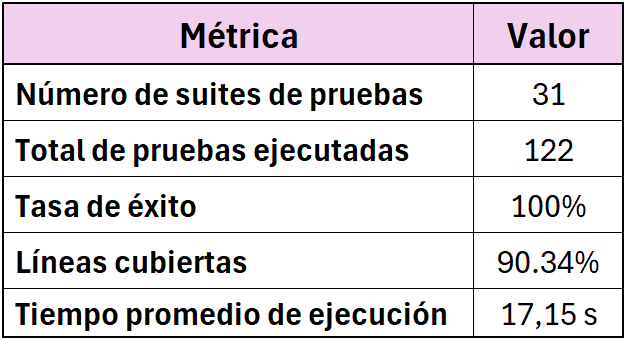
\includegraphics[width=0.5\textwidth]{figures/resultado_tests.png}
    \captionsetup{skip=7pt}
    \caption{Resultados globales de la ejecución de las pruebas.}
    \label{tab:resultado_tests}
\end{table}

\subsection{Interpretación de los Resultados}

La tasa de éxito del 100\% en las pruebas refleja que todas las verificaciones han pasado correctamente en cada ejecución. Sin embargo, \textbf{esto no significa que no se hayan encontrado problemas durante el desarrollo}. En varias ocasiones, los errores en los tests no estaban relacionados con fallos en la implementación de la aplicación, sino con limitaciones técnicas de Jest o con dependencias externas que dificultaban su correcta ejecución.

Uno de los principales obstáculos ha sido la incompatibilidad de ciertas librerías con Jest. Por ejemplo, los módulos basados en \textit{CommonJS}, como \texttt{D3.js}, han presentado dificultades en su integración con el entorno de pruebas. Además, los componentes que dependen de \texttt{canvas} no cuentan con soporte nativo en Jest, lo que impidió la ejecución de tests sobre algunos gráficos. Se intentó mitigar estos problemas mediante \textit{mocking} de dependencias, pero sin obtener resultados satisfactorios para todos los casos.

Aún así, la principal razón por la que se ha decidido suprimir los tests problemáticos ha sido por el flujo CI: Dado que está configurado en \textit{GitHub Actions} para ejecutar la suite de pruebas antes de cada despliegue en \textit{Vercel}, cualquier fallo en los tests bloquearía la actualización del código en producción. Para evitar interrupciones innecesarias en el despliegue debido a errores ajenos a la aplicación, se optó por retirar aquellas pruebas que no podían ofrecer resultados fiables sin comprometer la estabilidad del CI. A pesar de esta decisión, se ha garantizado que los tests implementados cubren los aspectos esenciales del sistema. Se han validado correctamente los endpoints del backend, la lógica de negocio y los principales componentes del frontend, asegurando que las funcionalidades críticas de la aplicación están correctamente verificadas. Para aquellos aspectos que no podían ser testeados automáticamente con Jest, como ciertos elementos gráficos o validaciones de autenticación, se han realizado pruebas manuales.

Finalmente, se ha trabajado en el tiempo de ejecución de las pruebas, logrando que la batería completa de 122 tests se ejecute en un promedio de 17.15 segundos. Este tiempo es aceptable, donde cada ejecución acumula tiempos entre la creación y configuración del entorno y la ejecución de los tests. Mantener este tiempo bajo control es un aspecto importarte en un flujo CI/CD.

\subsection{Cobertura del Código}

Por otro lado, también se ha utilizado la funcionalidad de cobertura de código de Jest para evaluar qué porcentaje del código está siendo verificado por los tests. La cobertura se mide en cuatro dimensiones:

\begin{itemize}
    \item \textbf{Statements}: Sentencias ejecutadas. \vspace{-5pt}
    \item \textbf{Branches}: Ramas de ejecución en estructuras de control (\textit{if/else}). \vspace{-5pt}
    \item \textbf{Functions}: Funciones llamadas. \vspace{-5pt}
    \item \textbf{Lines}: Líneas de código ejecutadas.
\end{itemize}

Los resultados en la tabla \ref{tab:coverage_tests} muestran que la mayoría de los archivos tienen una \textbf{cobertura superior al 90\%}, lo que indica que la mayor parte del código ha sido testeado de manera efectiva. No obstante, algunos archivos presentan una cobertura significativamente más baja:

\begin{itemize}
    \item \textbf{\texttt{app/api/auth/callback.ts}}: El archivo tiene una cobertura del 35.06\%. Esto se debe por el valor \texttt{state} que se utiliza para la protección ante ataques CSRF (\textit{Cross-Site Request Forgery}). Como no es el flujo de autenticación estándar, se genera un error \texttt{state\_mismatch} en todos los casos.
    \item \textbf{\texttt{components/stats/IndiceDeInterferencia.tsx}}:  Tiene una cobertura del 44.27\%, lo que indica que ciertas partes de la lógica de este componente aún no han sido probadas. En esta estadística es donde se hace uso de la librería D3.js, que genera problemas al no manejar módulos ESModules.
\end{itemize}

A pesar de estas limitaciones, la cobertura global es elevada y ha permitido validar el correcto funcionamiento de los principales módulos de la aplicación.

\begin{table}[htbp]
    \centering
    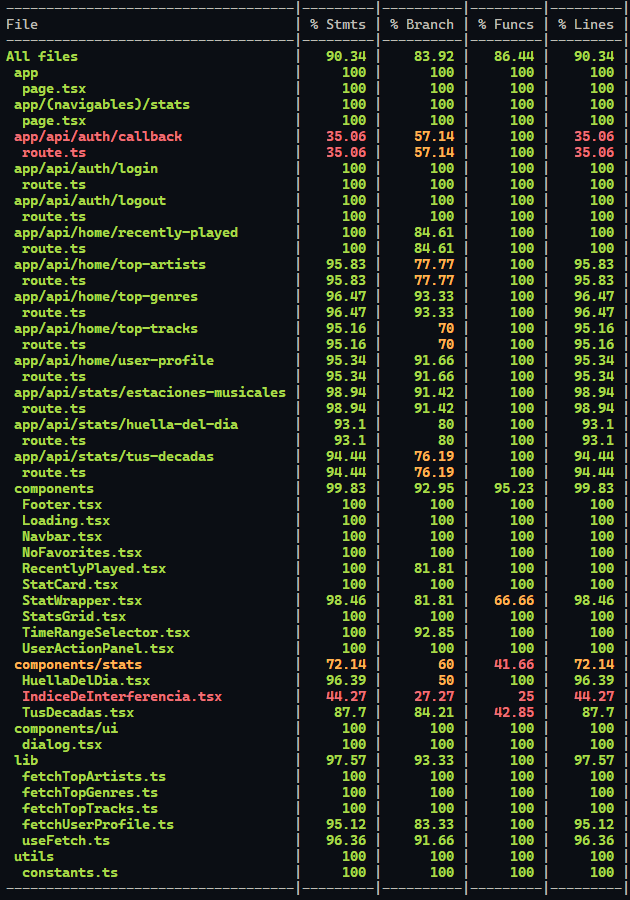
\includegraphics[width=0.6\textwidth]{figures/coverage_tests.png}
    \captionsetup{skip=7pt}
    \caption{Desglose generado por Jest de la cobertura del código del proyecto.}
    \label{tab:coverage_tests}
\end{table}


